\section{Μοντέλο dietz2011} \label{sec:dietz_theory}

Οι Dietz et al. κατασκεύασαν ένα μοντέλο της ανθρώπινης ακοής, με στόχο τον εντοπισμό της κατεύθυνσης ταυτόχρονων ομιλητών στο \cite{Dietz2011}. Ο άνθρωπος έχει μια ιδιαίτερα εύρωστη ικανότητα να εντοπίζει ήχους σε αντίξοες συνθήκες (αντήχηση, έντονος θόρυβος κλπ) οπότε κρίθηκε αναγκαίο να δημιουργηθεί ένα μοντέλο που προσομοιάζει τα χαρακτηριστικά του ανθρώπινου ακουστικού συστήματος με στόχο να χρησιμοποιηθεί αυτό σε αυτόματα συστήματα προσέγγισης DOA.

Η δομή του μοντέλου που κατασκευάστηκε χωρίζεται σε τρία μέρη. Το πρώτο κομμάτι, που θα απασχολήσει αυτή την ενότητα, είναι η ακουστική επεξεργασία για την εξαγωγή των ακουστικών παραμέτρων. Στο δεύτερο, εξάγονται τα σημαντικά τμήματα αυτών των παραμέτρων και στο τρίτο υλοποιείται το σύστημα εντοπισμού. 

\subsection{Ακουστική επεξεργασία}

Εδώ χρησιμοποιήθηκε το μοντέλο ακουστικής επεξεργασίας Interaural Phase Difference \cite{Dietz_2008}, και περιγράφεται παρακάτω.

\begin{enumerate}
    \item Προσεγγίζεται η χαρακτηριστική μεταφοράς του μέσου αυτιού (βλ. \ref{fig:auditory_system}), με ένα πρώτης τάξεως ζωνοπερατό φίλτρο $F_p = 500 Hz, F_c = 2 kHZ$.
    \item Το ακουστικό ζωνοπερατό φιλτράρισμα στην basilar μεμβράνη μοντελοποιείται με μια γραμμική, 4ης τάξης, τράπεζα φίλτρων που αποτελούνται μόνο από πόλους (gammatone filter-bank). Το πλάτος κάθε φίλτρου ορίζεται ως το ισοδύναμο τετραγωνικό εύρως ζώνης (Equivalent Rectangular Bandwidth - ERB) των ακουστικών φίλτρων. Υλοποιούνται 23 μπάντες φίλτρων στο διάστημα των 200 Hz - 5 kHz με απόσταση 1 ERB. Σημειώνεται πως το ERB είναι ένα μέτρο που χρησιμοποιείται στην ψυχοακουστική και δίνει μια εκτίμηση του εύρους ζώνης των φίλτρων στην ανθρώπινη ακοή, χρησιμοποιώντας μη ρεαλιστικά, αλλά βολικά μοντέλα τετραγωνικών ζωνοπερατών φίλτρων.
    \item Η συμπίεση του κοχλία λογιστικοποιήθηκε με άμεση συμπίεση ισχύος 0.4, μετά το bandpass φιλτράρισμα.
    \item Η διαδικασία της ηλεκτρομηχανικής μεταγωγής των εσωτερικών hair-cells, προσομοιώνεται με την ανόρθωση ημίσεος κύματος με διαδοχικά lowpass φίλτρα 5ης τάξης με $F_c = 770 Hz$.
    \item Οι αμφιωτικές χρονικές ανομοιότητες προκύπτουν από το ζωνοπερατό φιλτράρισμα με μιγαδικά gammatone φίλτρα 2ης τάξης.
\end{enumerate}{}

\noindent
Η μιγαδική έξοδος των φίλτρων (Εξίσωση \ref{eq:complex_filter_output}) περιέχει τη διαχωρίσιμη πληροφορία του πλάτους $\alpha(t)$ και της φάσης του σήματος $\phi(t)$.
\begin{CEquation}
    g(t) = \alpha(t) e^{i\phi(t)} \label{eq:complex_filter_output}
\end{CEquation}
Από τα αντίστοιχα αριστερά-δεξιά ζεύγη εξόδων των φίλτρων, $g_l$ και $g_r$, υπολογίζεται η αμφιωτική συνάρτηση μεταφοράς (Interaural Transfer Function - ITF) όπως φαίνεται στην Εξίσωση \ref{eq:ITF}.
\begin{CEquation}
    ITF(t) = g_l(t)\overline{g_r}(t) = 
    \alpha_l(t)\alpha_r(t) e^{i(\phi_l(t)-\phi_r(t))}
    \label{eq:ITF}
\end{CEquation}

Η ITF είναι μιγαδική και περιέχει και αυτή, την πληροφορία για τη φάση και για το πλάτος. Είναι άρα ιδανική για τη χρονική εξομάλυνση των αμφιωτικών συναρτήσεων. Η χρονικά εξομαλυμένη IPD εξάγεται στη συνέχεια από την ITF, αφού αυτή φιλτραριστεί από ένα χαμηλοπερατό φίλτρο, όπως φαίνεται στην Εξίσωση \ref{eq:IPD_extraction}
\begin{CEquation}
    IPD(t) = arg([ITF(t)]_{lp})
    \label{eq:IPD_extraction}
\end{CEquation}

Η IPD μπορεί να μετασχηματιστεί σε ITD διαιρώντας το IPD με την μέση άμεση συχνότητα του αριστερού και δεξιού σήματος. Ο τρόπος υπολογισμού της μέσης άμεσης συχνότητας φαίνεται στην Εξίσωση \ref{eq:instant_freq}

\begin{CEquation}
    f_{inst} = \frac{1}{4\pi}(\frac{d\phi_l(t)}{dt} + \frac{d\phi_r(t)}{dt})
    \label{eq:instant_freq}
\end{CEquation}

Τα μιγαδικά φίλτρα επιτρέπουν τον υπολογισμό της ITF και κατ' επέκταση την IPD της λεπτής-δομής (fine structure) ή της περιβάλλουσας (envelope) του σήματος. Το πρώτο επιτυγχάνεται με το κεντράρισμα του φίλτρου στην ίδια συχνότητα με το προηγούμενο ακουστικό φίλτρο. Για την περιβάλλουσα, το φίλτρο κεντράρεται, στη συχνότητα διαμόρφωσης ενδιαφέροντος, κατά προτίμηση, στην έξοδο του ακουστικού φίλτρου υψηλής συχνότητας. Το φίλτρο λεπτής δομής έχει Q-value 3, ενώ τα φίλτρα διαμόρφωσης έχουν Q-value 8.

Το ILD εκφράζεται σε dB, και πολλαπλασιάζεται με τον παράγοντα συμπίεσης c, όπου $c\sim0.4$ ,όπως φαίνεται στην εξίσωση \ref{eq:ILD_calc} ώστε να κλιμακωθεί η εσωτερική αναπαράσταση στο προτώτυπο ILD, που συμβαίνει στα αυτιά, πριν τη συμπίεση της basilar μεμβράνης.

\begin{CEquation}
    ILD(t) = 20clog_{10}(\frac{|h_r(t)|}{|h_l(t)|})
    \label{eq:ILD_calc}
\end{CEquation}

Το πλεονέκτημα αυτού του μοντέλου είναι η υψηλή φασματική ανάλυση των αμφιωτικών παραμέτρων, που μπορούν να υπολογιστούν δείγμα προς δείγμα. Ακόμα ένα πλεονέκτημα είναι το επιπλέον gammatone φιλτράρισμα που ακολουθεί το μοντέλο ηλεκτρομηχανικής μεταγωγής. Στα κανάλια χαμηλής συχνότητας (περίπου στο 1.4 kHz) ο βασικός λόγος ύπαρξης αυτών των φίλτρων είναι ο διαχωρισμός της DC συνιστώσας από την χρονική λεπτή δομή, όπως απαιτείται από τον υπολογισμό της φάσης. Στα κανάλια υψηλών συχνοτήτων, μπορούν να εφαρμοστούν παράλληλα φίλτρα με τη μορφή μιας τράπεζας φίλτρων διαμόρφωσης ή να προσαρμοστούν στην θεμελιώδη συχνότητα ή στον τόνο ενός συγκεκριμένου ομιλητή. Συνοπτικά το μοντέλο παρουσιάζεται στο Σχήμα \ref{fig:dietz_model_structure}

\begin{figure}[h]
  \centering
  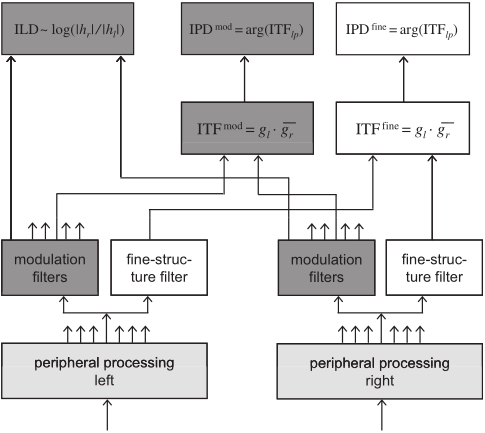
\includegraphics[width=\textwidth]{images/dietz_model_structure.png}
  \caption{Τα στάδια επεξεργασίας του ακουστικού μοντέλου. Η περιφερική επεξεργασία χωρίζει το σήμα εισόδου σε 23 ακουστικά φίλτρα ανά αυτί, και ακολουθείται από ανόρθωση ημίσεος κύματος, χαμηλοπερατό φιλτράρισμα και συμπίεση.}
  \label{fig:dietz_model_structure}
\end{figure}